\chapter{Appendix}
\label{ch:appendix}

\section{Source Code}

The scripts that were produced for the calculation of the metrics and the
analysis of the results are available in the following GitHub repository: \url{
    https://github.com/panos-span/custom_h5-index }

\subsection{General Scripts for all Metrics}

\textbf{Rank Order Correllation}

\lstinputlisting{../custom_h5-index/h5_index/rank_order_correlation.py}

\textbf{Average H5-Index of Cited Journals by ISSN}
\lstinputlisting{../custom_h5-index/h5_index/avg_h5_cited_issn.sql}

\lstinputlisting{../custom_h5-index/h5_index/avg_h5_mw.py}

\textbf{Citation Network Analysis}

\lstinputlisting{../custom_h5-index/h5_index/citation-graph_top_h5.py}

\lstinputlisting{../custom_h5-index/h5_index/mw_u.py}

\textbf{Traditional h-index calculation for authors}

\lstinputlisting{../custom_h5-index/h5_index/orcid_h5.sql}

\lstinputlisting{../custom_h5-index/h5_index/orcid_h5.rdbu}

\textbf{Adjusted h5-index calculation for authors}

\lstinputlisting{../custom_h5-index/h5_index/orcid_h5_filtered.sql}

\lstinputlisting{../custom_h5-index/h5_index/orcid_h5_filtered.rdbu}

\textbf{Adjusted h5-index calculation for authors from lower tier journals}

\lstinputlisting{../custom_h5-index/h5_index/orcid_h5_bottom.sql}

\lstinputlisting{../custom_h5-index/h5_index/orcid_h5_bottom.rdbu}

\textbf{H5 Index Calculation for Journals}

\lstinputlisting{../custom_h5-index/h5_index/issn_subject_h5.sql}

\lstinputlisting{../custom_h5-index/h5_index/issn_subject_h5.rdbu}

\textbf{Retrieve random works from hyperprolific authors}

\lstinputlisting{../custom_h5-index/h5_index/random_top_works_h5.sql}

\textbf{Retrieve random works from other authors}

\lstinputlisting{../custom_h5-index/h5_index/random_top_other_works_h5.sql}

\textbf{Works of Authors}

\lstinputlisting{../custom_h5-index/h5_index/works_orcid.sql}

\lstinputlisting{../custom_h5-index/h5_index/works_orcid.rdbu}

\textbf{Works with their respective ISSN and subject from ASJC codes}

\lstinputlisting{../custom_h5-index/h5_index/works_issn_subject.sql}

\lstinputlisting{../custom_h5-index/h5_index/works_issn_subject.rdbu}

\textbf{Work Citations}

\lstinputlisting{../custom_h5-index/h5_index/work_citations.sql}

\lstinputlisting{../custom_h5-index/h5_index/work_citations.rdbu}

\textbf{Top ISSNS by H5 Index (Same as JIF and EF)}

\lstinputlisting{../custom_h5-index/h5_index/top_issn_by_subject.sql}

\textbf{Filtered Works derived from the top ISSNs}

\lstinputlisting{../custom_h5-index/h5_index/filtered_works_orcid.sql}

\lstinputlisting{../custom_h5-index/h5_index/filtered_works_orcid.rdbu}

\textbf{Lower Quality ISSNs by H5 Index (Same as JIF)}

\lstinputlisting{../custom_h5-index/h5_index/bottom_issn_by_subject.sql}

\textbf{Filtered Works derived from the lower quality ISSNs}

\lstinputlisting{../custom_h5-index/h5_index/bottom_filtered_works_orcid.sql}

\lstinputlisting{../custom_h5-index/h5_index/bottom_filtered_works_orcid.rdbu}

\subsection{Ranking Journals based on the JIF of 3 years}

\textbf{JIF Index Calculation for Journals}

\lstinputlisting{../custom_h5-index/impact_factor/impact_factor.sql}

\lstinputlisting{../custom_h5-index/impact_factor/impact_factor.rdbu}

\textbf{Citable Works}

\lstinputlisting{../custom_h5-index/impact_factor/citable_works.sql}

\lstinputlisting{../custom_h5-index/impact_factor/citable_works.rdbu}

\textbf{Citations}

\lstinputlisting{../custom_h5-index/impact_factor/citations.sql}

\lstinputlisting{../custom_h5-index/impact_factor/citations.rdbu}

\textbf{Publications in the Impact Factor Period}

\lstinputlisting{../custom_h5-index/impact_factor/publications.sql}

\subsection{Ranking Journals based on the EigenFactor of 5 years}

\textbf{Citation Network}

\lstinputlisting{../custom_h5-index/impact_factor/citation_network.sql}

\textbf{EigenFactor Calculation for Journals}

\lstinputlisting{../custom_h5-index/eigenfactor/eigenfactor.py}

\textbf{Lower Quality ISSNs by EigenFactor}

\lstinputlisting{../custom_h5-index/eigenfactor/bottom_issn_by_subject.sql}

\section{Dependency Graphs}
The full dependency graph of the h index calculations can be seen in Figures
\ref{fig:dependency_graph_h5}, \ref{fig:dependency_graph_jif}, and
\ref{fig:dependency_graph_ef}.

\begin{figure}[H]
    \centering
    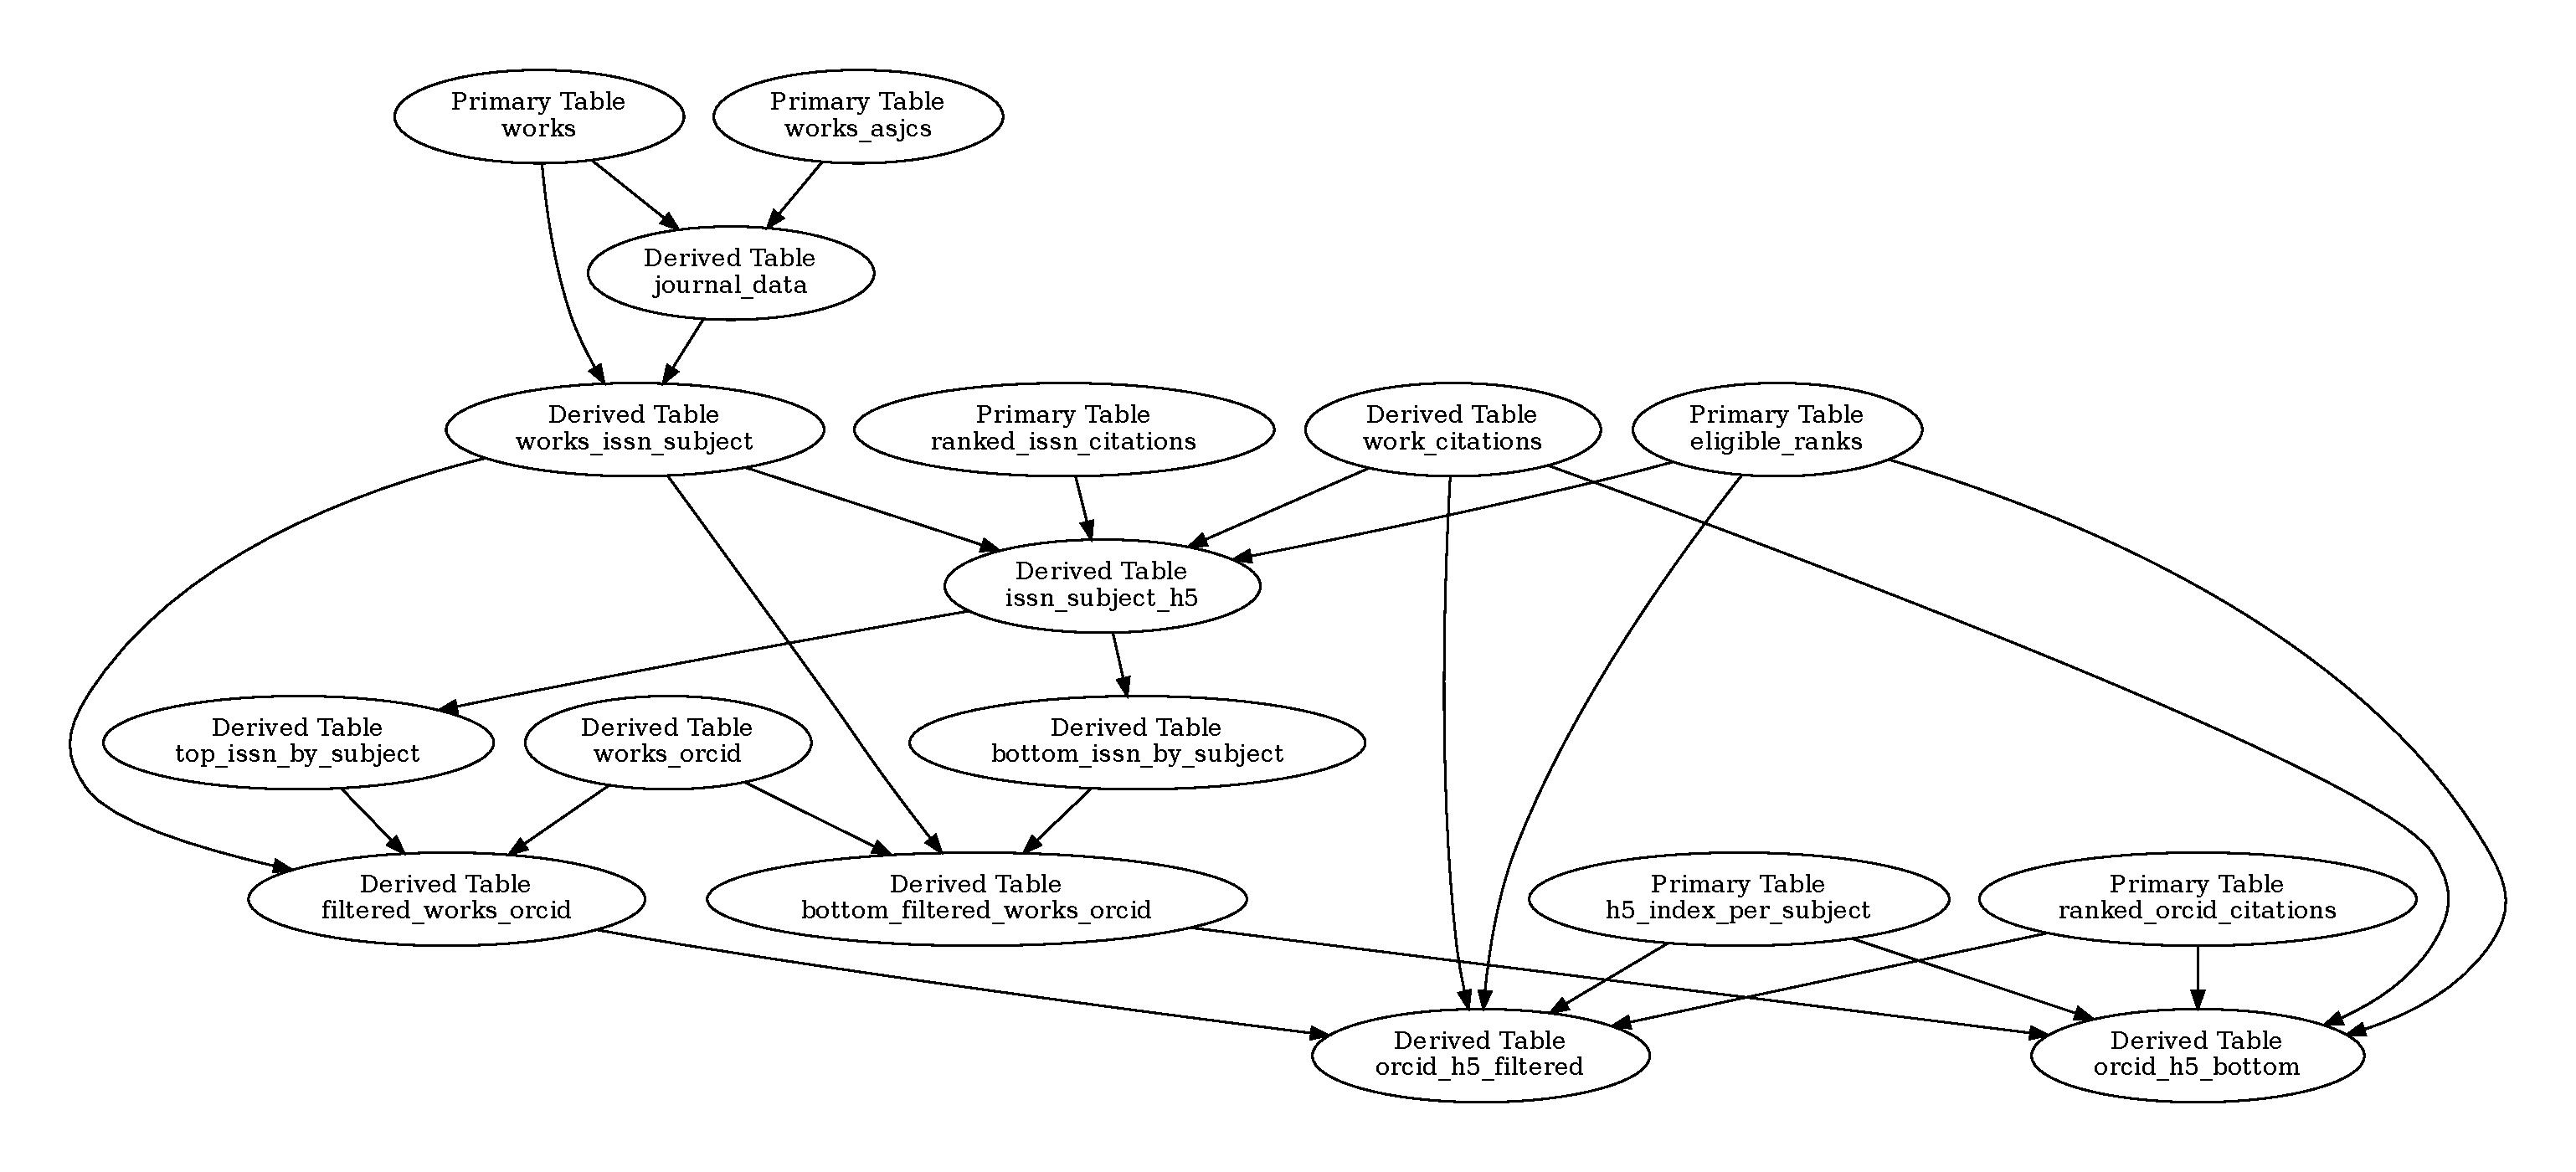
\includegraphics[width=\textwidth]{../figs/full-graph_h5.pdf}
    \caption{Full Dependency graph of the adjusted h5-index calculation with journals filtered using the h5-index}
    \label{fig:dependency_graph_h5}
\end{figure}

\begin{figure}[H]
    \centering
    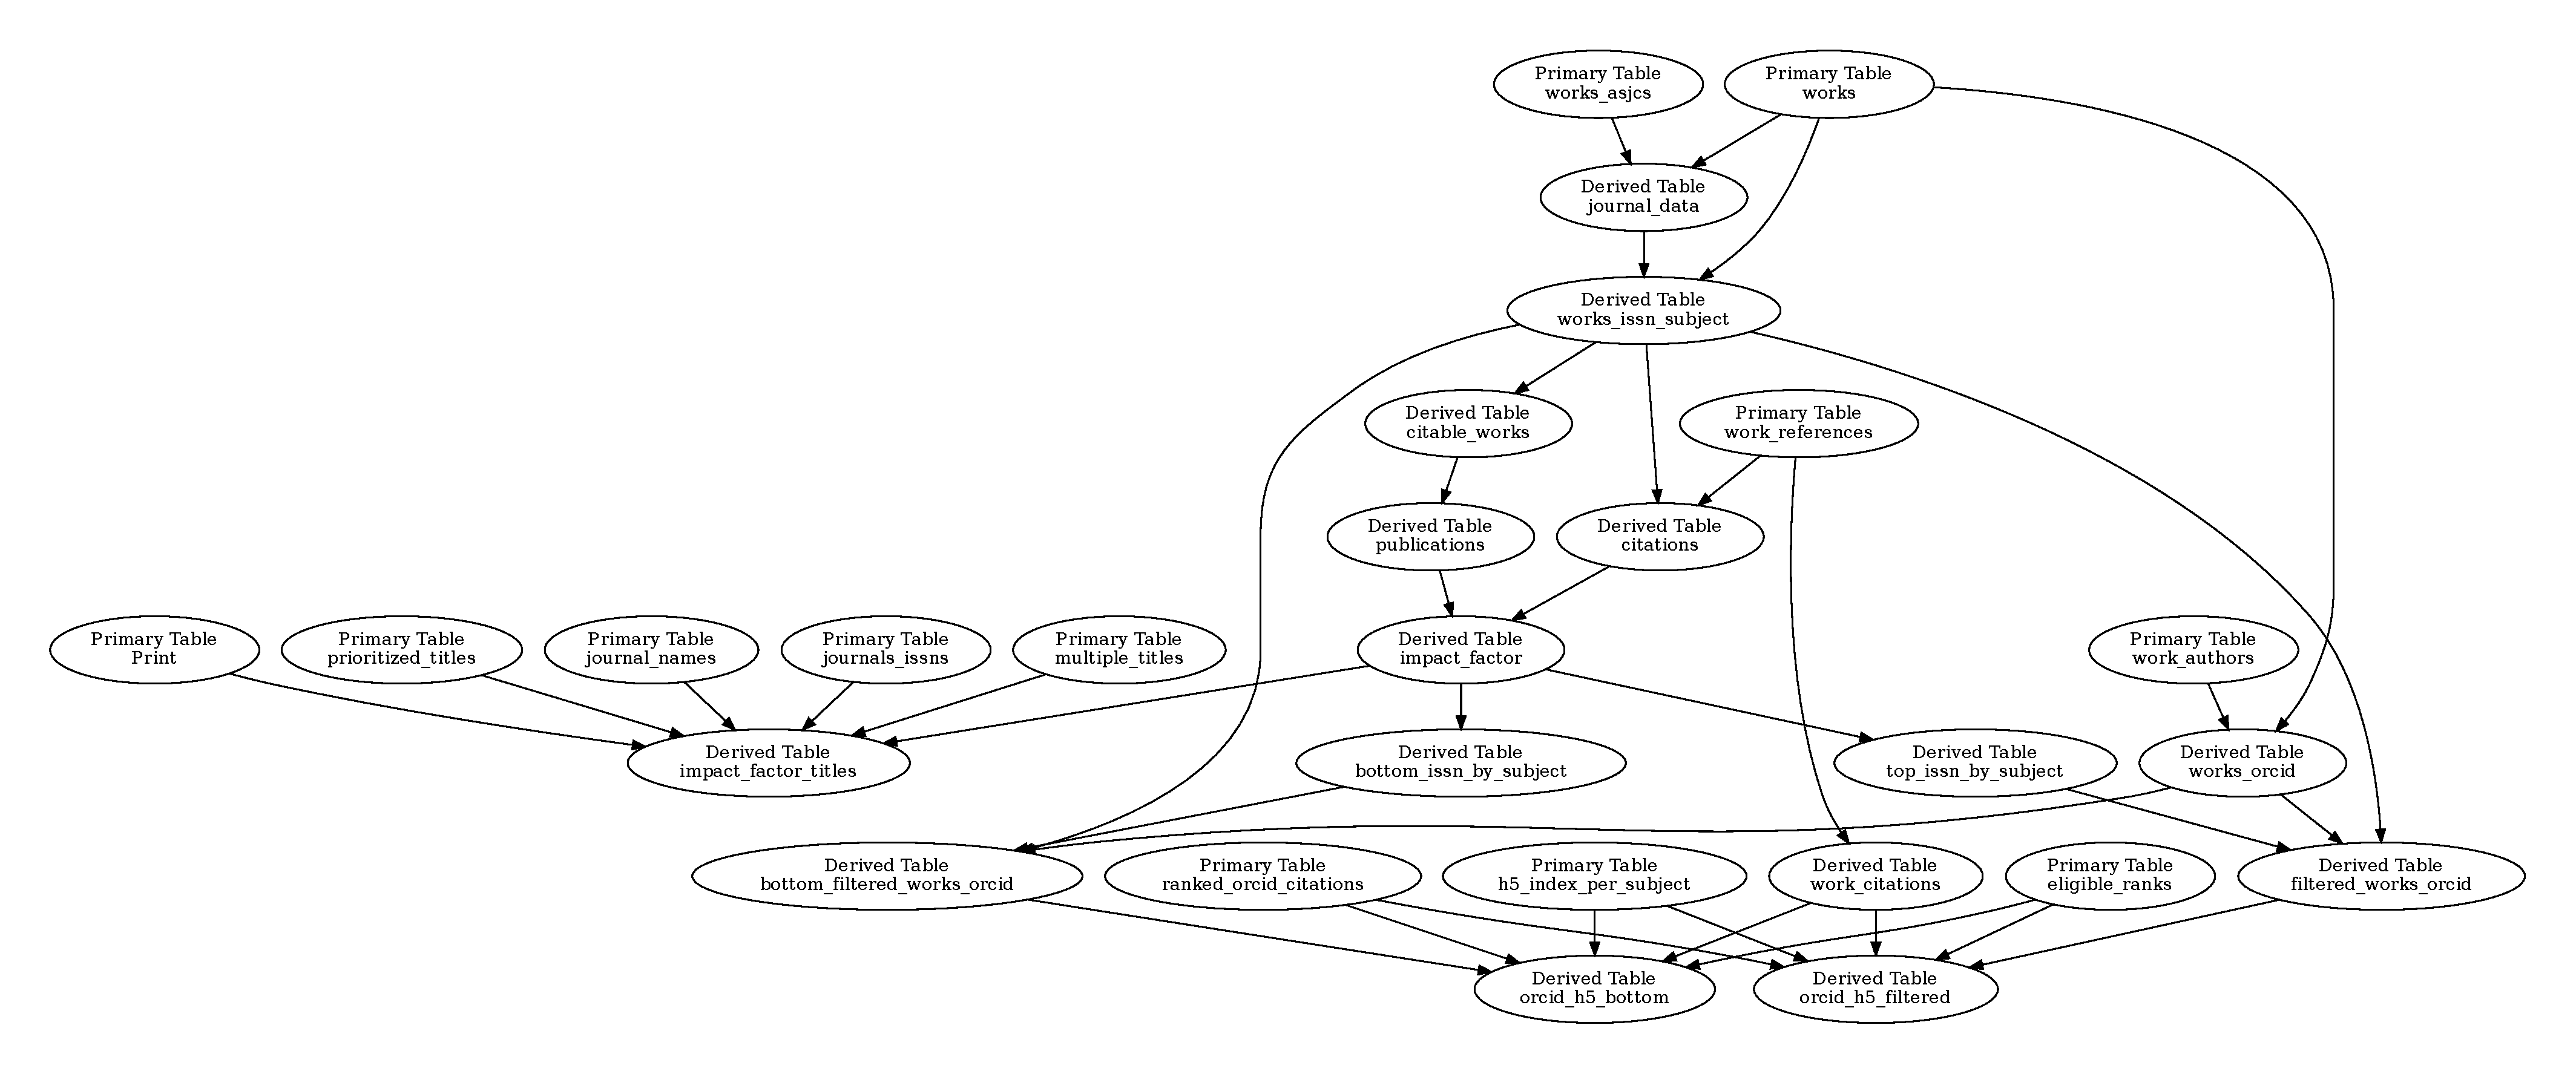
\includegraphics[width=\textwidth]{../figs/full-graph_jif.pdf}
    \caption{Full Dependency graph of the adjusted h5-index calculation with journals filtered using the impact factor}
    \label{fig:dependency_graph_jif}
\end{figure}

\begin{figure}[H]
    \centering
    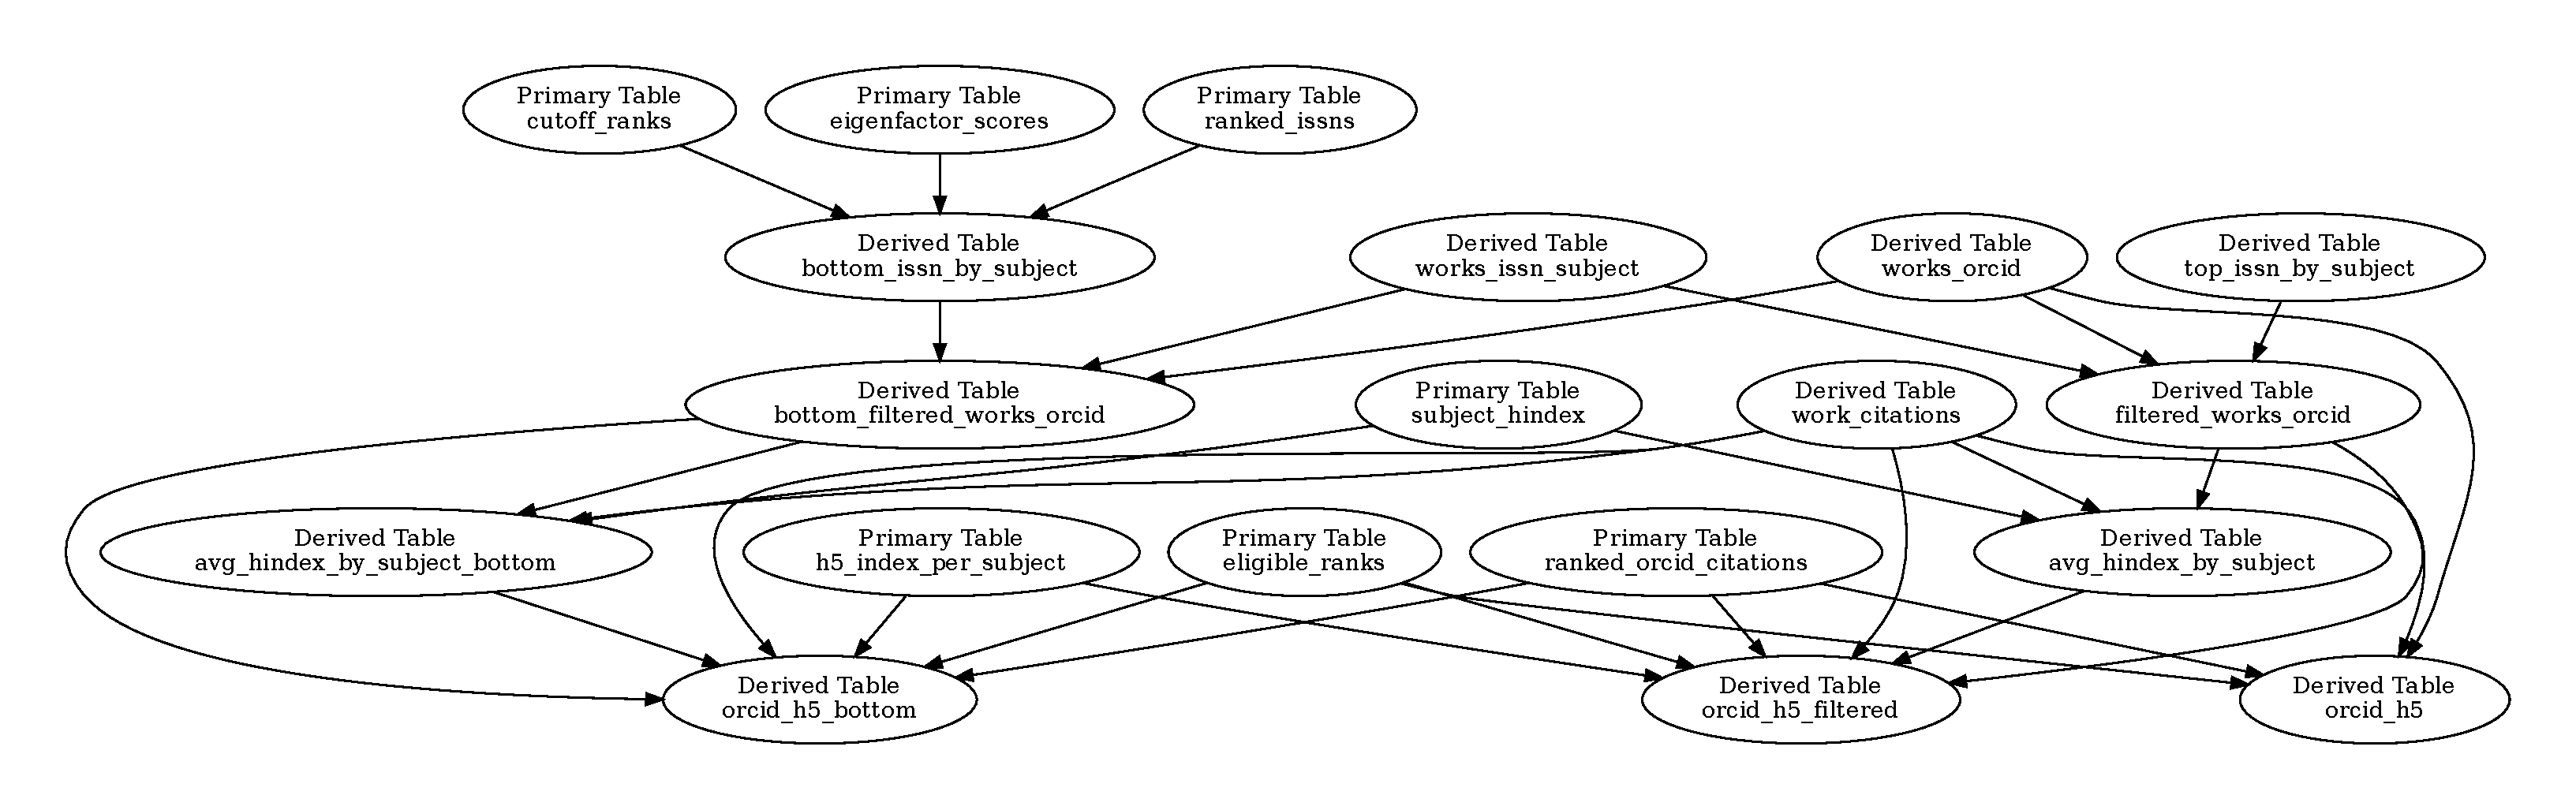
\includegraphics[width=\textwidth]{../figs/full-graph_ef.pdf}
    \caption{Full Dependency graph of the adjusted h5-index calculation with journals filtered using the EigenFactor}
    \label{fig:dependency_graph_ef}
\end{figure}

